%% ═══════════════════════════════════════════════════════════════════════════
\section{The Repair and Its Re-measurement}
%% ═══════════════════════════════════════════════════════════════════════════
\label{app:repair}
%% ═══════════════════════════════════════════════════════════════════════════

The campaign identified one defect and specified one repair, which was then carried out and
re-measured against the identical frozen campaign. The declarations, the scenario and the event
script are unchanged and the same 120 forecasts are recomputed by the modified model, so every
difference below belongs to the model and to nothing else.

\subsection{The Repair That Was Recommended Does Not Work}

Section~\ref{sec:res_discussion} proposed making the calibrated events write a lead-time
impact. Implemented and measured, that repair fails, and the reason is the one
Figure~\ref{fig:completion_repair} draws: a completion date estimated as a full production
cycle beginning now multiplies the lead time by the fraction of work remaining, so a quantity
routed into the lead time is scaled by that fraction too. On NovaFab, the node carrying the
scenario's accident, the four-week probability fell from $0.846$ to $0.000$ on a milestone
that was in fact missed.

\begin{figure}[htbp]
    \centering
    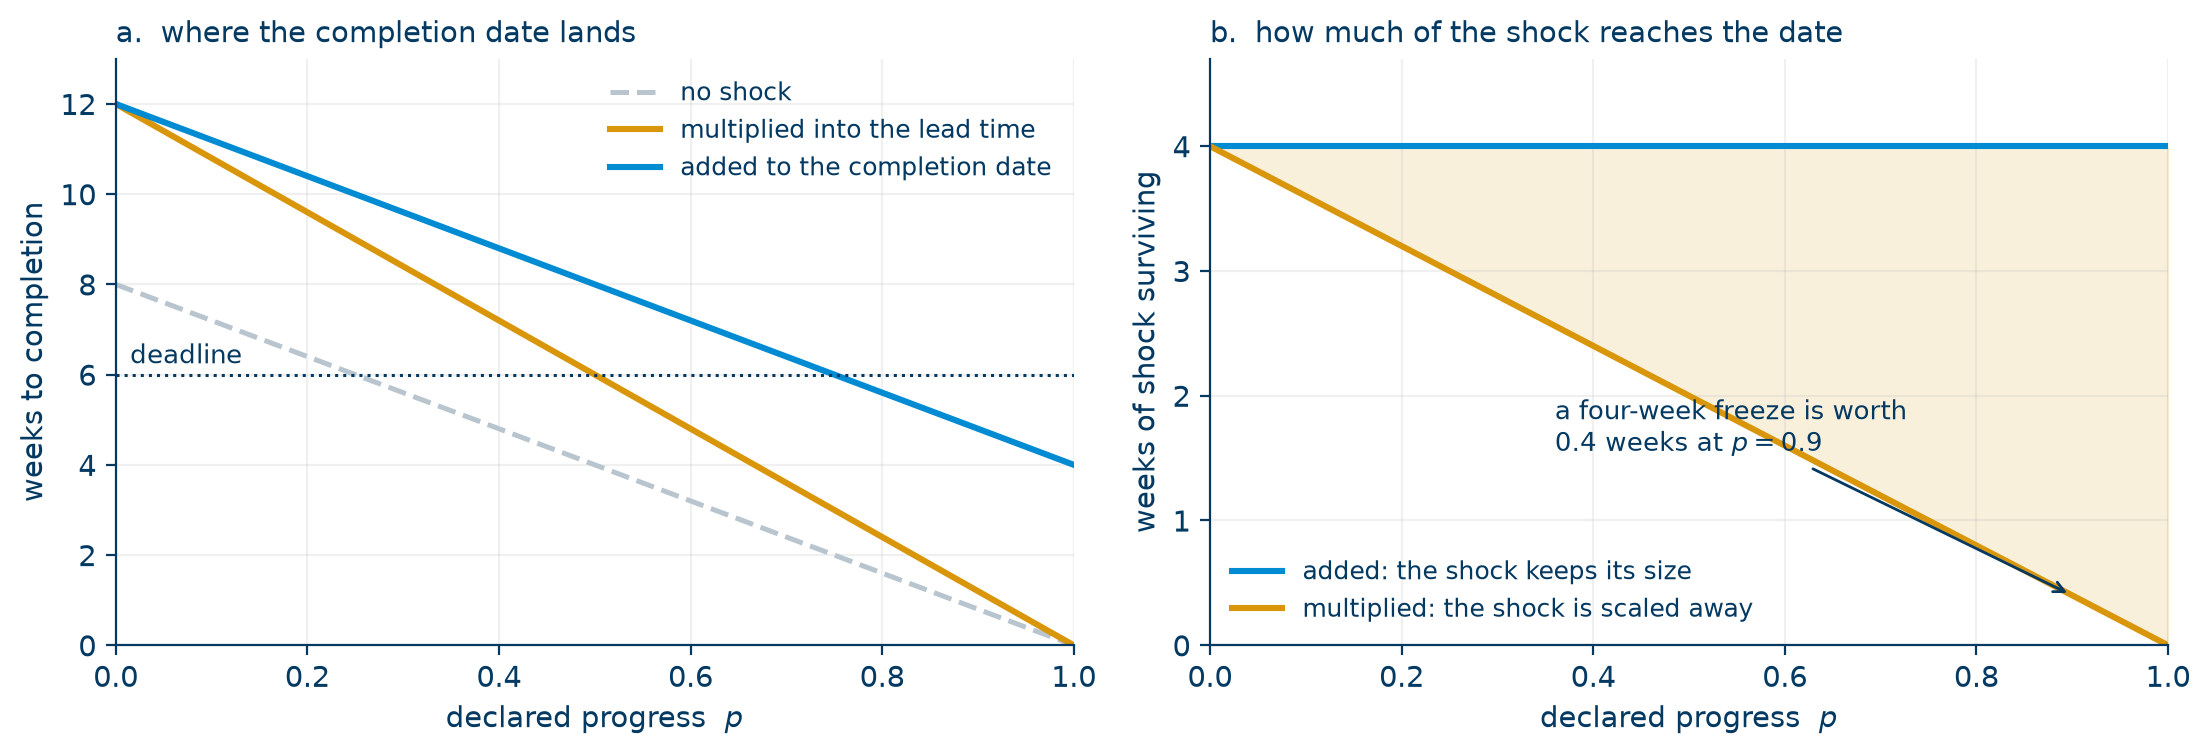
\includegraphics[width=\linewidth]{Images/completion_repair.png}
    \caption[Why the obvious repair fails]{The two repairs on one milestone, with a nominal
    lead time of eight weeks and four weeks lost to a shock. Routing the lost time through the
    lead time (ochre) scales it by the work remaining, so a four-week freeze is worth $3.6$
    weeks at a tenth complete and $0.4$ weeks at nine tenths; adding it to the completion date
    (azure) keeps its size throughout. The milestones on which the two disagree most are those
    nearest their deadline, which are precisely those on which a warning has value.}
    \label{fig:completion_repair}
\end{figure}

The completion model was rewritten accordingly, identically in the three independent
estimators the system carries for the same quantity, the analytic $u_{\text{time}}$ block, the
Monte Carlo forecast rollout and the PERT lead-time simulator:
\begin{equation}
    C \;=\; t \;+\; (1 - p)\,L \;+\; R,
    \label{eq:completion_repaired}
\end{equation}
where $p$ is the declared progress, $L$ the lead time and $R$ the time already lost. Five
families of capacity-halting event, machine failure, accident, strike weighted by the share
of workforce involved, material shortage weighted by criticality, and cyber incident, now
accumulate their effective duration into $R$. Loss of storage capacity deliberately does not,
since it removes space rather than production hours.

The mechanical effect is unambiguous. Where the accumulated-delay field was written a non-zero
value exactly zero times across the whole of arm A, after the repair NovaFab accumulates
$154.7$ engine hours at its first shock and $371.2$ over the campaign, carried in 27 of its 41
snapshots.

\subsection{Two Further Defects Exposed by the First}

With the time block responsive, a second defect became measurable. The milestone-miss
probability returned exactly $0$ or exactly $1$ in $85.0\%$ of the 120 forecasts, leaving 14
anywhere in between: a switch rather than a probability, as two declarants recorded in free
text before it was measured. The cause is that the rollout drew the lead time at random while
taking declared progress as an exact value. Declared progress is the least reliable input the
system receives and belongs to precisely the class of quantity the framework exists to doubt,
so the forecast layer was treating as certain a figure the adequacy score is built to suspect.
Progress is now drawn per replicate, with a standard deviation widened node by node in
proportion to that node's own measured hidden risk $H$, so the system's adequacy measurement
feeds its own forecast.

The third defect was in the data rather than the model, and it would have invalidated any
calibration performed before it was found. Indicator coverage on the campaign database was
$25.6\%$: 24 of the 42 indicators were empty on all eight nodes, the carbon and cost blocks
were inert everywhere, and only three of the six urgency blocks contributed. The lead time
itself was present on five nodes of eight, and the remaining three received a risk floor of
zero through the documented fallback for a missing lead time, which is an absence of data
presenting itself as a reassuring prediction. Completing the indicators from public figures
of the 2020 to 2022 shortage raised coverage to $49.1\%$ and made all six blocks active. One
model bug was undetectable until then: a per-node recovery capability, a 26-week aerospace
requalification time, was being read as production time already lost, pinning that node's
time block at $1.0$ from the first turn. An empty database conceals the errors of the model
that consumes it, which is a methodological point independent of this framework.

\subsection{The Re-measurement}

Table~\ref{tab:repair_scores} scores the recomputed forecasts against the original-commitment
definition of Section~\ref{sec:res_target_trap}, at all four horizons, on the same censored
samples of 112, 104, 96 and 90 observations. The middle column of each pair isolates the
structural repair; the right-hand column adds the progress-uncertainty term.

\begin{table}[htbp]
\centering
\caption{The frozen campaign rescored after repair, original-commitment target}
\label{tab:repair_scores}
\small
\begin{tabularx}{\linewidth}{c *{6}{>{\centering\arraybackslash}X}}
\toprule
& \multicolumn{3}{c}{\textbf{Brier skill}} & \multicolumn{3}{c}{\textbf{AUC}} \\
\cmidrule(lr){2-4}\cmidrule(lr){5-7}
\textbf{Horizon} & before & structure & + uncertainty & before & structure & + uncertainty \\
\midrule
1 week  & $-1.278$ & $-0.646$ & $-0.687$ & 0.736 & 0.793 & 0.729 \\
2 weeks & $-0.690$ & $-0.401$ & $-0.367$ & 0.636 & 0.671 & 0.634 \\
3 weeks & $-0.654$ & $-0.360$ & $-0.286$ & 0.641 & 0.657 & 0.602 \\
4 weeks & $-0.553$ & $-0.272$ & $-0.216$ & 0.654 & 0.721 & 0.584 \\
\bottomrule
\end{tabularx}
\end{table}

\begin{figure}[htbp]
    \centering
    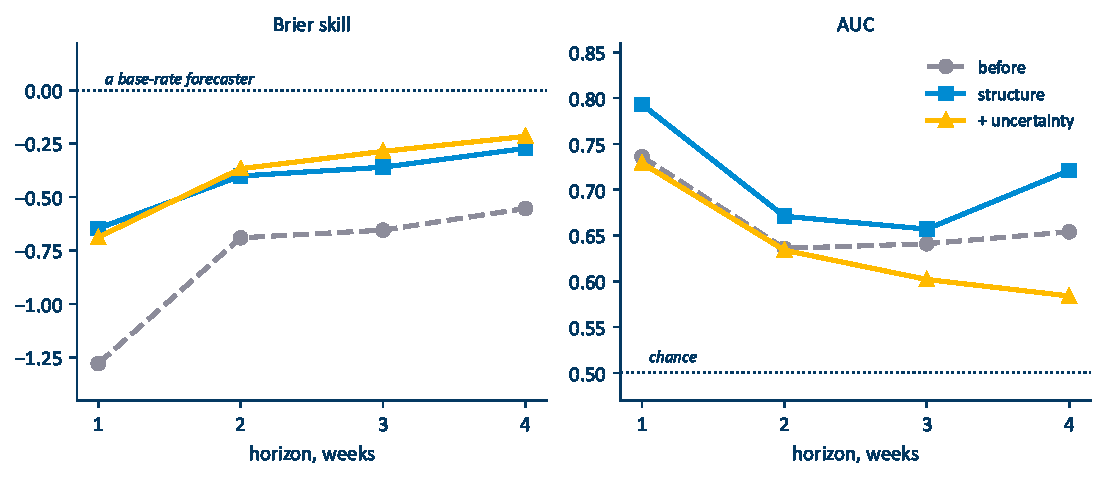
\includegraphics[width=\linewidth]{Images/repair_effect.pdf}
    \caption[What the repair bought and what it traded]{The same three model versions on both
    metrics. The structural repair lifts calibration and discrimination together. The
    progress-uncertainty term then lifts calibration further at every horizon beyond one week
    and lowers discrimination at every horizon, which is a trade rather than a gain and is why
    it was retained on the calibration evidence rather than on the AUC.}
    \label{fig:repair_effect}
\end{figure}

The structural repair improves both axes at every horizon without trading one for the other,
which is the clean result of this thesis's second measurement campaign. The
progress-uncertainty term is a trade rather than a gain, and the AUC movement it costs is not
interpretable. With 26
positive observations the cluster-bootstrap interval on the four-week AUC runs from $0.21$ to
$0.87$ and contains every value in its row, and the same objection that bounds the original
discrimination claim of Section~\ref{sec:res_armA_scored} bounds this one. The term was
retained on the calibration evidence and on the argument that a declared quantity should not
enter a probabilistic forecast as a certainty, not on the AUC.

Three qualifications belong beside the table. The Brier skill remains negative at every
horizon, so the forecast is still worse calibrated than a forecaster that announces the base
rate and stops; the repair moves the system from badly wrong to less wrong, not to useful.
The milestone probability remains binary in $71.7\%$ of cases against $85.0\%$ before, so the
over-confidence is reduced rather than removed. And the post-hoc calibration layer that
Section~\ref{sec:res_discussion} recommended was trained, measured, and deliberately not
connected: on the synthetic factory that produced its training data it improves the Brier
skill by $30.8\%$ and the AUC from $0.792$ to $0.850$, but applied to the campaign it improves
calibration at every horizon while dropping the four-week AUC from $0.721$ to $0.580$. Its
training label is an event striking the node at exactly $t+1$; the product displays a missed
milestone or a critical event cumulated over $(t, t+4]$. The layer cannot rank the cases
driven by the milestone channel because it has never seen one. This is the trap of
Section~\ref{sec:res_target_trap} encountered from the opposite direction: a calibration
fitted against the wrong target degrades a system that works, exactly as an evaluation
against the wrong target can condemn one. Connecting the layer requires the training label to
be rebuilt on the product's target, which requires the synthetic factory's snapshots to
record milestone truth, which they do not; that is the next concrete step rather than an
open research question.

\subsection{A Third Arm, and What It Does Not Show}

The repaired system was then exercised through a full nineteen-turn campaign in closed loop,
in which the same eight agents no longer only declared but also selected actions from a fixed
catalogue, applied to the chain by the mutation service and recorded in the intervention
journal: promote a backup arc, replan a milestone, expedite a shipment, raise capacity, revise
a declaration, or do nothing. One hundred and fifty-two declarations were recorded with no
unresolved consistency failure. The anti-contamination protocol of
Section~\ref{sec:methods_controls} was tightened for this arm: every message reaching an agent
is written by the tool into that agent's own sandbox, and a failed consistency check is
answered with the interface's own guidance rather than with a coordinator's instruction.

\begin{figure}[htbp]
\centering
\begin{tikzpicture}[x=1cm, y=1cm, font=\scriptsize,
    arm/.style  = {bloc, text width=3.0cm, minimum height=0.85cm},
    met/.style  = {minimum width=0.52cm, minimum height=0.52cm, draw=altenNavy,
                   line width=0.5pt, fill=altenAzure!35},
    miss/.style = {minimum width=0.52cm, minimum height=0.52cm, draw=altenNavy,
                   line width=0.5pt, fill=white},
    swap/.style = {minimum width=0.52cm, minimum height=0.52cm, draw=altenOchreDark,
                   line width=1.2pt, fill=altenOchrePale}]

\node[arm] (a) at (1.9, 1.5) {\textbf{arm A}\\declaration only};
\node[arm, blocFort] (c) at (1.9, -0.3) {\textbf{arm C}\\declarants act};

%% arm A meets milestones 1..5
\foreach \i in {1,2,3,4} {
  \pgfmathsetmacro{\x}{4.5 + 0.66*(\i-1)}
  \node[met] at (\x, 1.5) {};
}
\node[swap] at (6.48, 1.5) {};                      % the one arm C replans away
\foreach \i in {6,7,8,9,10,11} {
  \pgfmathsetmacro{\x}{4.5 + 0.66*(\i-1)}
  \node[miss] at (\x, 1.5) {};
}

%% arm C keeps four, loses the fifth, gains the sixth
\foreach \i in {1,2,3,4} {
  \pgfmathsetmacro{\x}{4.5 + 0.66*(\i-1)}
  \node[met] at (\x, -0.3) {};
}
\node[miss] at (6.48, -0.3) {};
\node[swap] at (7.14, -0.3) {};                     % the one arm C saves
\foreach \i in {7,8,9,10,11} {
  \pgfmathsetmacro{\x}{4.5 + 0.66*(\i-1)}
  \node[miss] at (\x, -0.3) {};
}

\node[etiquette, anchor=west, fill=none] at (11.7, 1.5) {5 of 11 met};
\node[etiquette, anchor=west, fill=none] at (11.7, -0.3) {5 of 11 met};

\draw[flecheCoupee] (6.48, 1.15) -- (6.48, 0.42) -- (7.14, 0.42) -- (7.14, 0.05);
\node[etiquette, anchor=south, text=altenOchreDark, text width=4.4cm] at (9.4, 0.28)
     {one replanned that would have held, one genuinely saved};

\node[etiquette, anchor=north, text width=12cm] at (7.0, -1.0)
     {the same count, and not the same five: acting on the signal changes \emph{which}
      commitment is met rather than \emph{how many}, and with eleven milestones neither the
      benefit nor the cost is statistically established};

\end{tikzpicture}
\caption[The third arm changes which, not how many]{Milestones met on their original
commitment, arm~A against arm~C on the repaired system. The totals are identical and the sets
are not: the two ochre squares are the swap. That is the effect a human campaign would need
to be powered to detect.}
\label{fig:third_arm}
\end{figure}

The headline figure flatters the framework and should not be used: six of eleven milestones
were missed in the frozen scenario and none was left unfinished in the closed loop, which reads
as six saved. Against the original commitments it is not, and Figure~\ref{fig:third_arm} gives
the honest count. The saved milestone is an electronics series delivered on its original date
that had slipped in the frozen truth. Beyond the swap, four late deliveries became replannings
announced in advance rather than slips discovered at the deadline, which has value to a customer
without being a save. Both the benefit and the cost are reported as facts of one campaign rather
than as results.

Two observations from that arm do carry. The arm B disarming reproduced exactly, eight
agents of eight at first exposure. And the causal chain the campaign showed to be broken now
closes: where arm A's foundry manager recorded that the tool was holding a low position
through a widely reported crisis and took no action, the repaired run moved the same node's
four-week probability from $0.088$ to $0.214$ at the shock turn and the agent replanned its
milestone. One reserve on internal validity must be stated: the model changed twice during
that campaign, at turns 15 and 16, so turns 16 to 18 are not comparable with what precedes
them. Every behavioural observation reported above is drawn from turns strictly earlier than
15.

\subsection{A Hypothesis That Became Measurable Again}

The criticality index degenerates under saturation, which forced H3 to be judged on the ten informative turns of nineteen and the other nine to be excluded. That exclusion rule is no longer necessary. The ranking now carries a log-survival key, $\ell(p) = -\ln(1-p)$ computed on an $\varepsilon$-regularised twin of the same propagation, which orders identically to $\Delta U_r$ outside saturation, a property-based invariant with a test to match, and keeps separating nodes inside it.

Re-measured on the repaired run, the two criteria decompose cleanly on the same data. The old criterion alone leaves 10 informative turns with NovaFab top-1 on 9 of them; adding the $\Delta \ell$ key leaves 17 informative turns of 19 with NovaFab top-1 on 16, a share of $94\%$ against a pre-registered threshold of $80\%$. Holding the criterion fixed instead and changing only the model, the frozen campaign gives $70\%$ and the repaired one $90\%$, so completing the indicators moves the figure as much as the new key does.

This is reported as exploratory and does not re-decide H3, for the same reason given for H4 in Section~\ref{sec:hypothesis_status}: a hypothesis re-run against a changed model no longer tests what the register asked, and two things changed at once here. Only the comparison of the two criteria on one run isolates a single cause. The defensible claim is the narrow one: the degeneracy that made nearly half the campaign unreadable is largely gone, and the quantity H3 tests now sits above its threshold on the repaired system.


%% ═══════════════════════════════════════════════════════════════════════════
